% !TEX encoding = UTF-8 Unicode

%
% Exemple de rapport
% par Pierre Tremblay, Universite Laval
% modifié par Christian Gagne, Universite Laval
% modifié par Francis Valois, Université Laval
% 31/01/2011 - version 1.4
%

%
% Modele d'organisation d'un projet LaTeX 
% rapport/      dossier racine et fichier principal
% rapport/fig   fichiers des figures\textbf{•}
% rapport/tex   autres fichiers .tex
%

% ** Preambule **
%
% Ajouter les options au besoin :
%    - "ULlof" pour inclure la liste des figures, requis si "\begin{figure}" utilise
%    - "ULlot" pour inclure la liste des tableaux, requis si "\begin{table}" utilise
%
\documentclass[12pt,ULlof,ULlot]{ULrapport}

% Chargement des packages supplementaires (si absent de la classe)
\usepackage[utf8]{inputenc}
\usepackage[T1]{fontenc}
\usepackage[autolanguage]{numprint}
\usepackage{icomma}
\usepackage{subfigure}
\usepackage{graphicx}
\usepackage[absolute]{textpos}
\usepackage[final]{pdfpages}
\usepackage{float}
%\usepackage[framed,numbered,autolinebreaks,useliterate]{mcode}
\def\dbar{{\mathchar'26\mkern-12mu d}} 
%\usepackage[options]{nom_du_package}

% Definition d'une commande pour presenter des cellules multilignes dans un tableau
\newcommand{\cellulemultiligne}[1]{\begin{tabular}{@{}c@{}}#1\end{tabular}}


% Definition de colonnes en mode paragraphe avec alignement ajustable
% Cette definition requiert le chargement du package "array"
%    - alignement horizontal, parametre #1 : - \raggedright (aligne a gauche)
%                                            - \centering (centre)
%                                            - \raggedleft (aligne a droite)
%    - alignement vertical, parametre #2 : - p (aligne en haut)
%                                          - m (centre)
%                                          - b (aligne en bas)
%    - largeur, parametre #3 : longueur
\newcolumntype{Z}[3]{>{#1\hspace{0pt}\arraybackslash}#2{#3}}

% Definitions des parametres de la page titre
\TitreProjet{Rapport de laboratoire 4}                         % Titre du projet
\TitreRapport{Transmission des ondes électromagnétiques}       % Titre du rapport
\Destinataire{M. Dominique Grenier}         % Nom(s) du destinataire
\TableauMembres{%                                     % Tableau des membres de l'equipe
   910\,055\,897  & Daniel Thibodeau \\\hline
   910\,097\,879  & Francis Valois \\\hline        % matricule & nom & \\\hline
           % matricule & nom & \\\hline     % matricule & nom & \\\hline
}
\DateRemise{20 novembre 2012}                           % Date de remis


% Corps du document

\begin{document}

%   Chapitres
%%!TEX root = ../rapport.tex
%!TEX encoding = UTF-8 Unicode

% Chapitres "Introduction"

% modifié par Francis Valois, Université Laval
% 31/01/2011 - version 1.0 - Création du document

\chapter{Introduction}
\label{s:introduction}

%!TEX root = ../rapport.tex
%!TEX encoding = UTF-8 Unicode

% Chapitres "Introduction"

% modifié par Francis Valois, Université Laval
% 31/01/2011 - version 1.0 - Création du document


\label{s:experimentation}
\chapter{Laboratoire 2}
\section{Projet 1}
Nous avons choisi une charge de valeur 100$\Omega$ puisque pour cette valeur, on obtient un coefficient de réflexion théorique faible. Pour affirmer cela, on utilise l'expression suivante:
\begin{equation}
\Gamma_g (s) = \frac{Z_g(s) - Z_0(s)}{Z_g(s) + Z_0(s)}\label{eq:reflex}
 \end{equation} 

\paragraph{}Dans le circuit étudié, on cherche à avoir $Z_0$ (l'impédance mise en parallèle avec la source) $\approx Z_G$ (l'impédance de la ligne)

\paragraph{}Afin d'observer de manière pratique le comportement des réflexions du circuit, nous avons essayé chacune des résistance disponible dans les choix en plus de celle de 100$\Omega$. Nous présenterons les courbes obtenus à l'oscilloscope à l'annexe \ref{s:annexes}. Comme seule la courbe pour la résistance de 100$\Omega$ est requise selon l'énoncé de laboratoire, elle est présentée ci-dessous:

\begin{figure}[htb]
\begin{center}
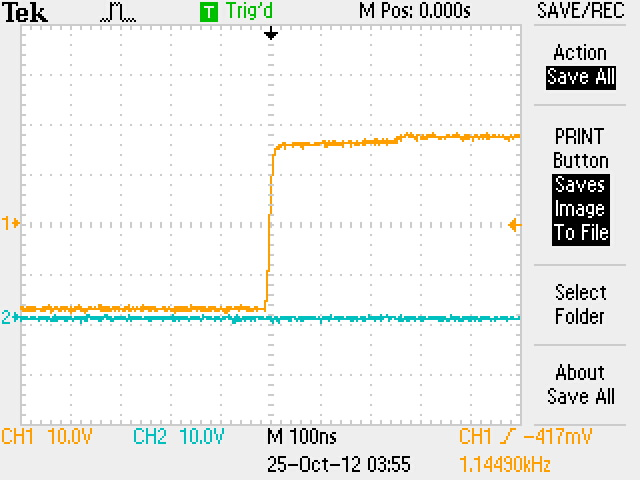
\includegraphics[scale=0.3]{Reflexion_R_100.jpg}
\caption{Courbes obtenus à l'oscilloscope pour le projet 1 en utilisant une résistance de 100 $\Omega$}
\label{Reflexion_R_100}
\end{center}
\end{figure}

On note dans cette figure que la réflexion est bel et bien faible, mais existante, en utilisant une résistance variable (le potentiomètre), on lit au multimètre une résistance très proche de 93$\Omega$. Cette résistance est très proche de l'impédance intrinsèque de ligne du tableau 1 présenté dans le protocle de laboratoire( $z_0 = 93\Omega$). L'ensemble des autres courbes est présenté dans l'annexe \ref{s:annexes}

\paragraph{}On remarque que la valeur fournie par le manufacturier est très précise. La différence entre la valeur du manufacturier et celle mesurée repose sur le bruit du signal qui affecte la précision de la lecture à l'oscilloscope et aussi la précision limitée de l'instrument de mesure de la résistance. 

\paragraph{}Pour ce qui est de déterminer la longueur de ligne, nous avons que la première réflexion vue à la source pour une résistance de 27 $\Omega$ est vue à une différence de temps (par rapport à la montée initiale) de $\approx 250ns$. Or, ce temps correspond au temps d'aller-retour. Afin de déterminer la longueur de la ligne, on divise par deux le temps d'aller-retour, ce qui donne 125ns et puis, on divise la vitesse de propagation par ce temps. Soit $v_p = 0.86 \times c \left[\frac{m}{s}\right]$, $l \left[m\right] = 0.86\times c \left[\frac{m}{s}\right] \times 125 ns = 37.475 \left[m\right]$. La ligne de transmission fait donc 37.475$\left[m\right]$ de long.

\section{Projet 2}

Dans ce projet, il était demandé de visualiser simultanément les signaux au niveau de la charge et de la source sur la ligne RG-58 de 30m. Cela fut fait pour des charges de respectivement 0 $\Omega$, 27 $\Omega$ et 50$\Omega$. Les courbes obtenues sont présentées à la section suivante.
\subsection{Présentation des courbes obtenues expérimentalement}
\begin{figure}[htb]
	\centering
\subfigure[Régime transitoire pour $R = 0 \Omega$]{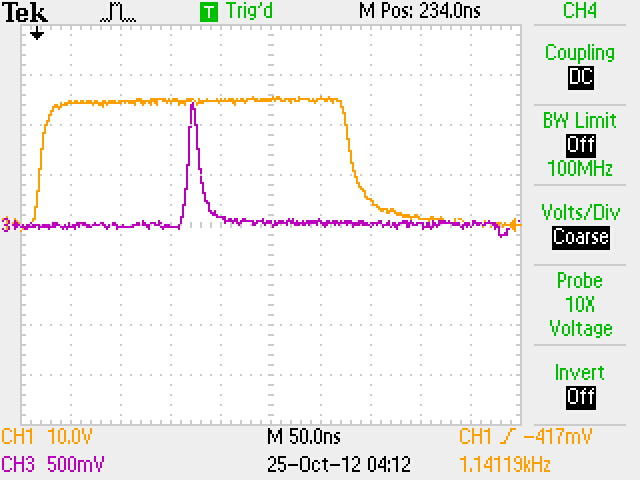
\includegraphics[scale =0.3]{fig/TR0.JPG} \label{fig:transr0}}
		\quad
		\subfigure[Front montant du régime transitoire pour $R = 27 \Omega$]{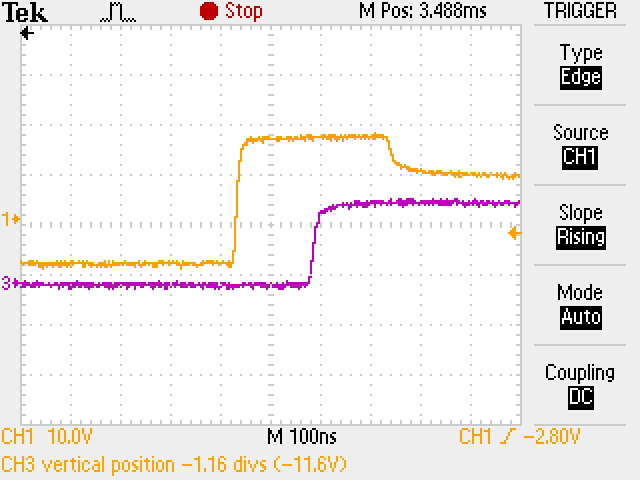
\includegraphics[scale =0.3]{fig/TR272.JPG} \label{fig:transr272}}
		\quad
		\subfigure[Front descendant du régime transitoire pour $R = 27 \Omega$]{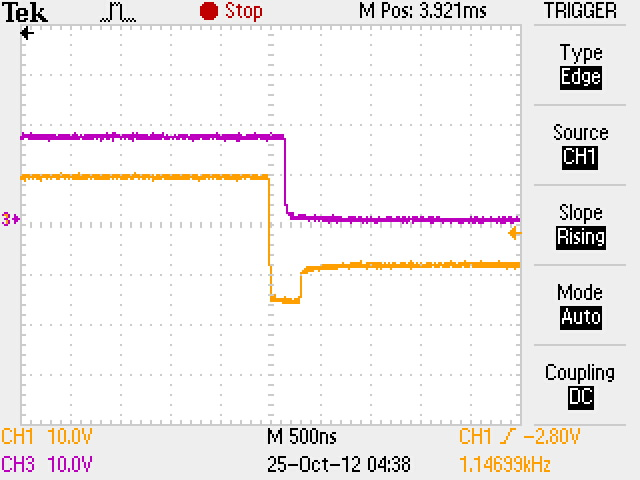
\includegraphics[scale =0.3]{fig/TR271.JPG} \label{fig:transr271}}
		\quad
		\subfigure[Vue d'ensemble du régime transitoire pour $R = 27 \Omega$]{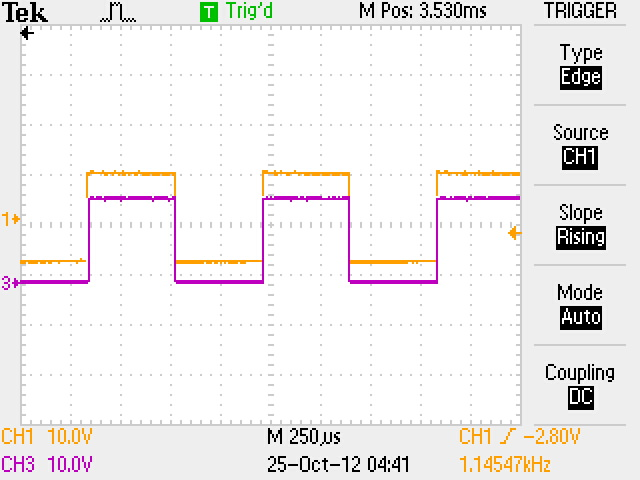
\includegraphics[scale =0.3]{fig/TR273.JPG} \label{fig:transr273}}
\end{figure}

\setcounter{subfigure}{0}
\begin{figure}[htb]
	\centering
\subfigure[Front montant du régime transitoire pour $R = 50 \Omega$]{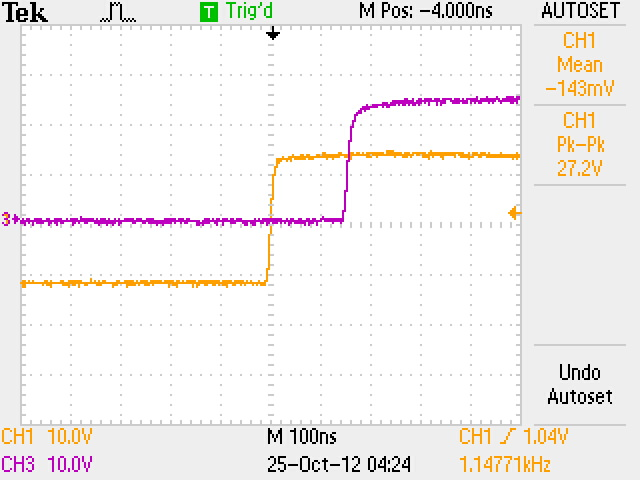
\includegraphics[scale =0.3]{fig/TR501.JPG} \label{fig:transr501}}
		\quad
		\subfigure[Front descendant du régime transitoire pour $R = 50 \Omega$]{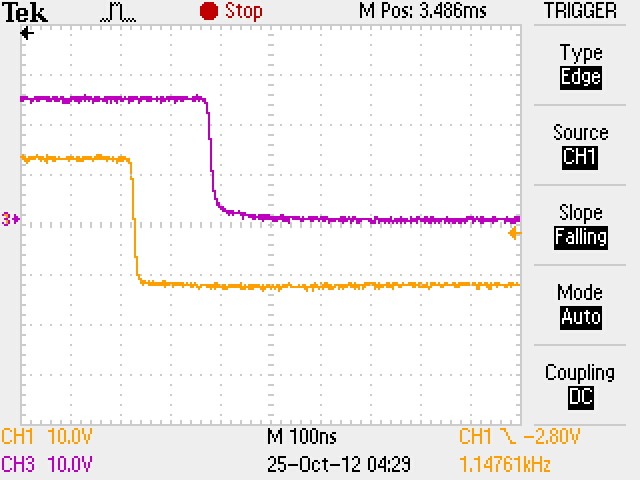
\includegraphics[scale =0.3]{fig/TR502.JPG} \label{fig:transr502}}
		\quad
		\subfigure[Vue d'ensemble du régime transitoire pour $R = 50 \Omega$]{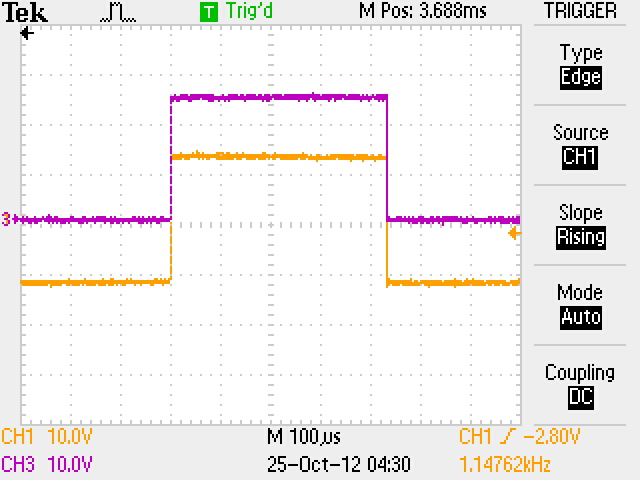
\includegraphics[scale =0.3]{fig/TR503.JPG} \label{fig:transr503}}
\end{figure}
\newpage
\subsection{Présentation des calculs}
Un example de chacun des calculs demandés est présenté ci-dessous.
L'équation utile au calcul du coefficient de réflexion est présentée à l'équation \ref{eq:reflex}. 
\subsubsection*{Calcul du coefficient de réflexion vu par la source}
Le développement du calcul du coefficient de réflexion vu par la source est présenté ci-dessous:
\begin{align}
\Gamma_g (s) &= \frac{Z_g(s) - Z_0(s)}{Z_g(s) + Z_0(s)}\\
		 &= \frac{50 - 50 }{50 + 50}\notag\\
		 &= 0\notag
\end{align}
\subsubsection*{Calcul de la tension $V^{+}(s)$}
On note premièrement sur la figure \ref{fig:transr501} que la tension de la source était de 27.2 V.
\begin{align}
V^{+}(s) &=  \frac{Z_0}{Z_0 + R_g} V_g (s)\\
		 &=	 \frac{50}{50 + 50} 27.2 \notag\\
		 &=  13.6V\notag
\end{align}

\subsubsection*{Calcul des coefficients de réflexion vus aux charges}
\begin{equation}
\Gamma_c (s) = \frac{Z_c(s) - Z_0(s)}{Z_c(s) + Z_0(s)}
\end{equation}
\textbf{Pour R = $0\Omega$}
\begin{align*}
\Gamma_c (s) &= \frac{Z_c(s) - Z_0(s)}{Z_c(s) + Z_0(s)}\\
			 &= \frac{0 - 50 }{0 + 50}\\
			 &= -1
\end{align*}
\textbf{Pour R = $27\Omega$}
\begin{align*}
\Gamma_c (s) &= \frac{Z_c(s) - Z_0(s)}{Z_c(s) + Z_0(s)}\\
			 &= \frac{27 - 50 }{27 + 50}\\
			 &= -0.2987
\end{align*}
\textbf{Pour R = $50\Omega$}
\begin{align*}
\Gamma_c (s) &= \frac{Z_c(s) - Z_0(s)}{Z_c(s) + Z_0(s)}\\
			 &= \frac{50 - 50 }{50 + 50}\\
			 &= 0
\end{align*}
\newpage
\subsection{Présentation des courbes théoriques}
Les courbes théoriques utiles pour l'analyse et la discussion sont présentées ci-dessous.
\setcounter{subfigure}{0}
\begin{figure}[htb]
	\centering
\subfigure[Régime transitoire théorique pour $R = 0 \Omega$]{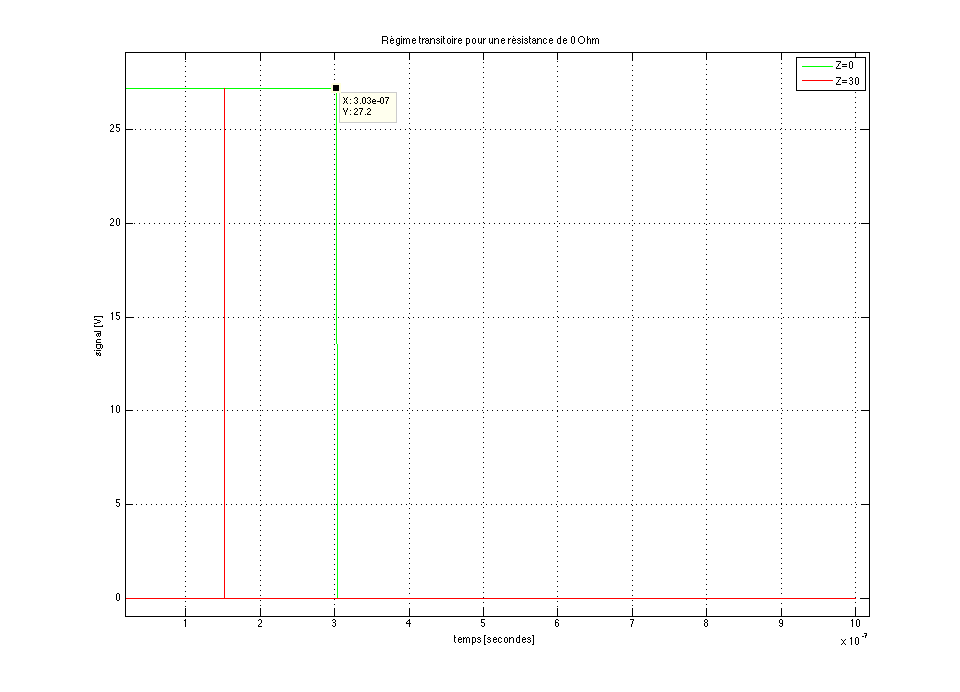
\includegraphics[scale =0.2]{fig/r0.png} \label{fig:r0}}
		\quad
		\subfigure[Régime transitoire théorique pour $R = 27 \Omega$]{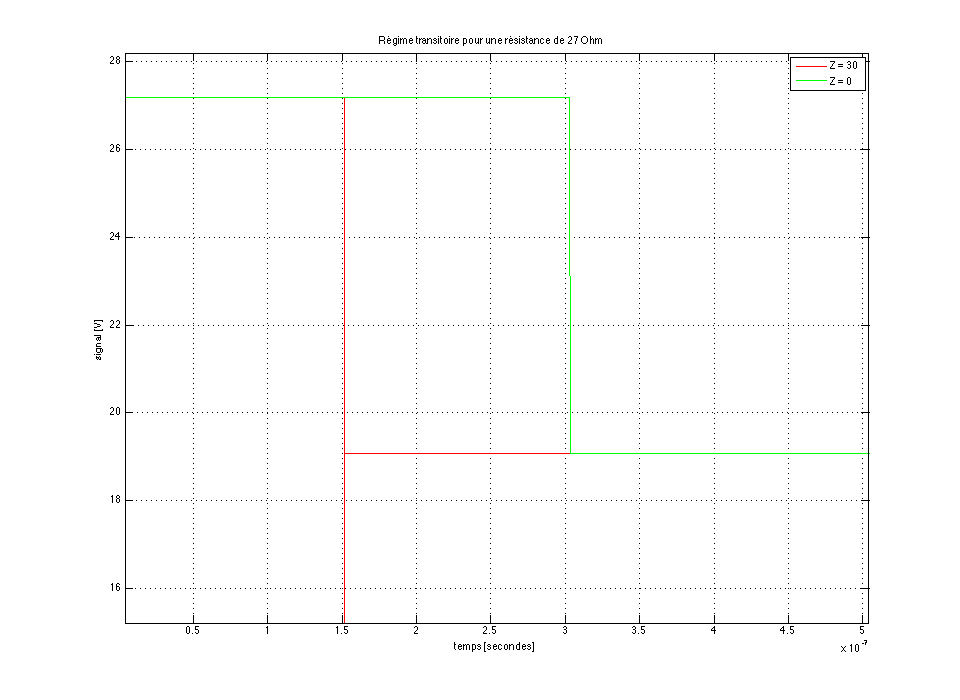
\includegraphics[scale =0.2]{fig/r27.png} \label{fig:r27}}
		\quad
		\subfigure[Régime transitoire théorique pour $R = 50 \Omega$]{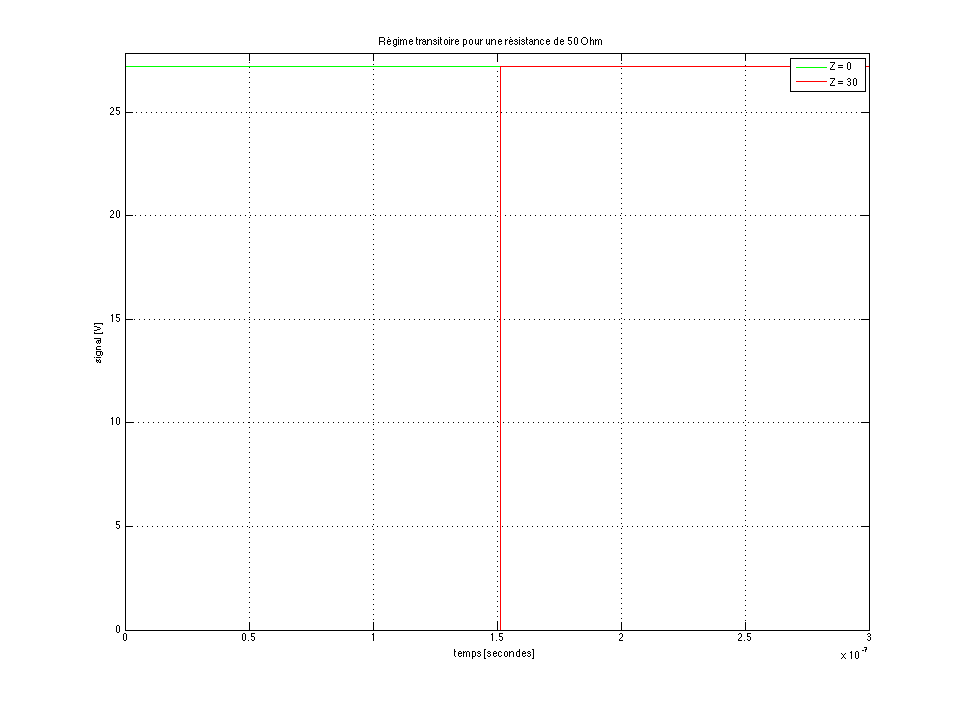
\includegraphics[scale =0.2]{fig/r50.png} \label{fig:r50}}
\end{figure}


\newpage
\setcounter{subfigure}{0}
\begin{figure}[htb]
	\centering
\subfigure[Diagramme en z pour $R = 0 \Omega$]{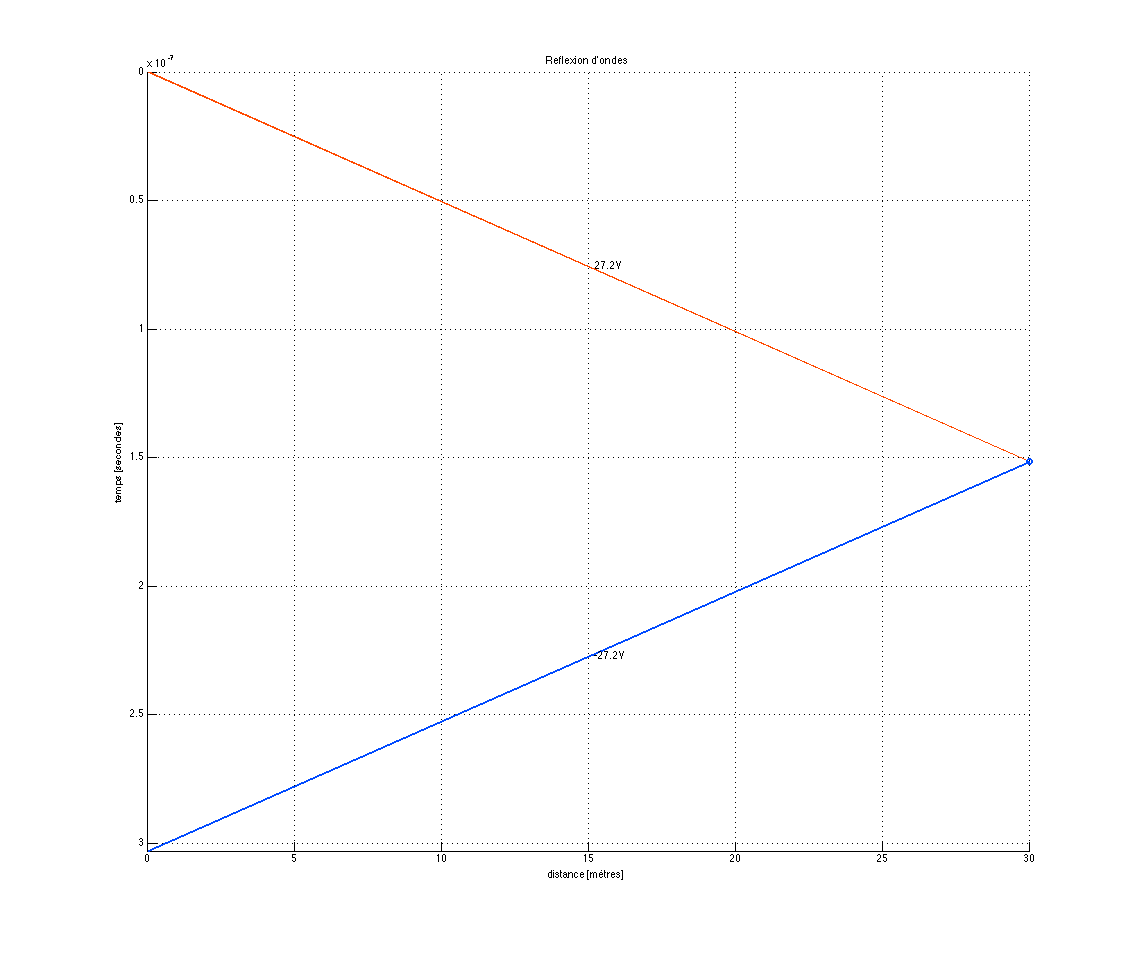
\includegraphics[scale =0.15]{fig/zr0.png} \label{fig:zr0}}
		\quad
		\subfigure[[Diagramme en z pour $R = 27 \Omega$]{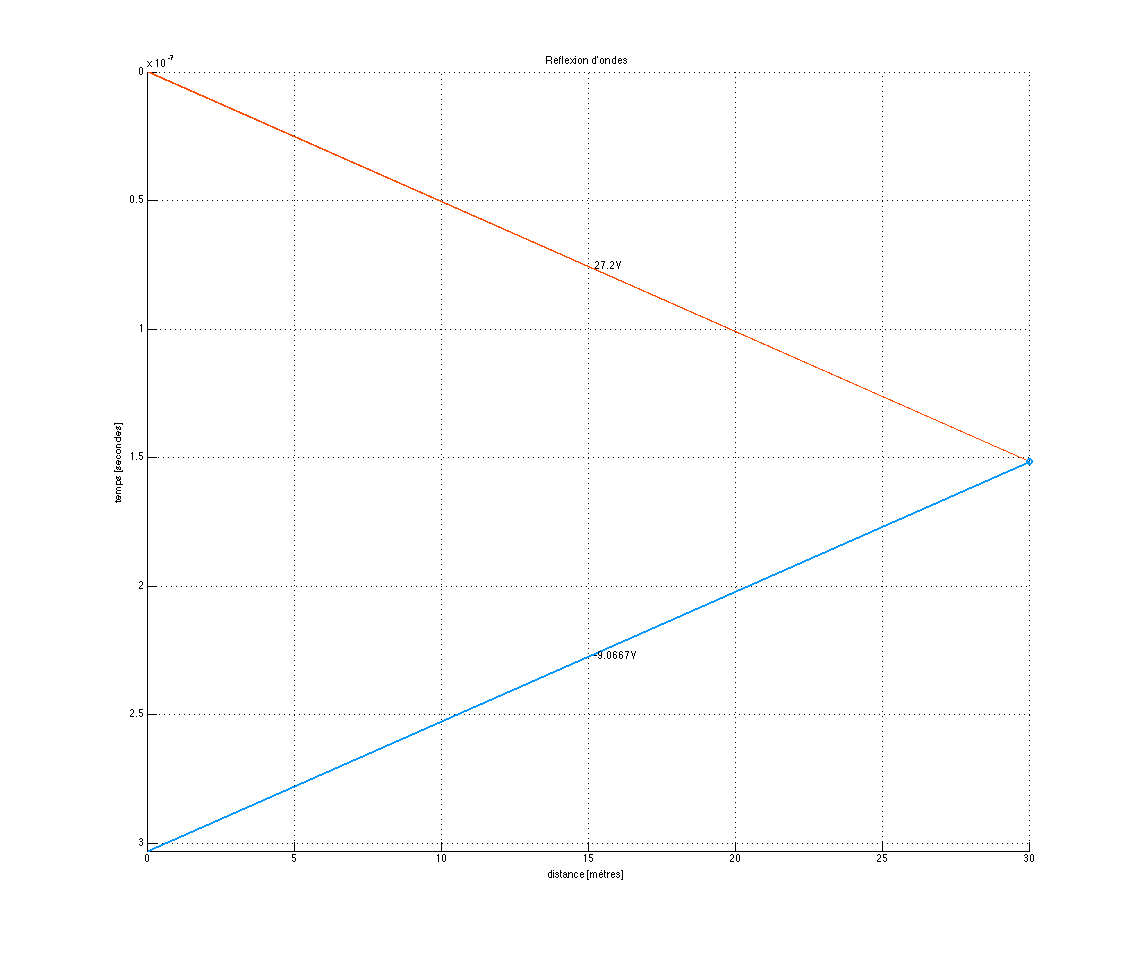
\includegraphics[scale =0.15]{fig/zr25.png} \label{fig:zr25}}
		\quad
		\subfigure[[Diagramme en z pour $R = 50 \Omega$]{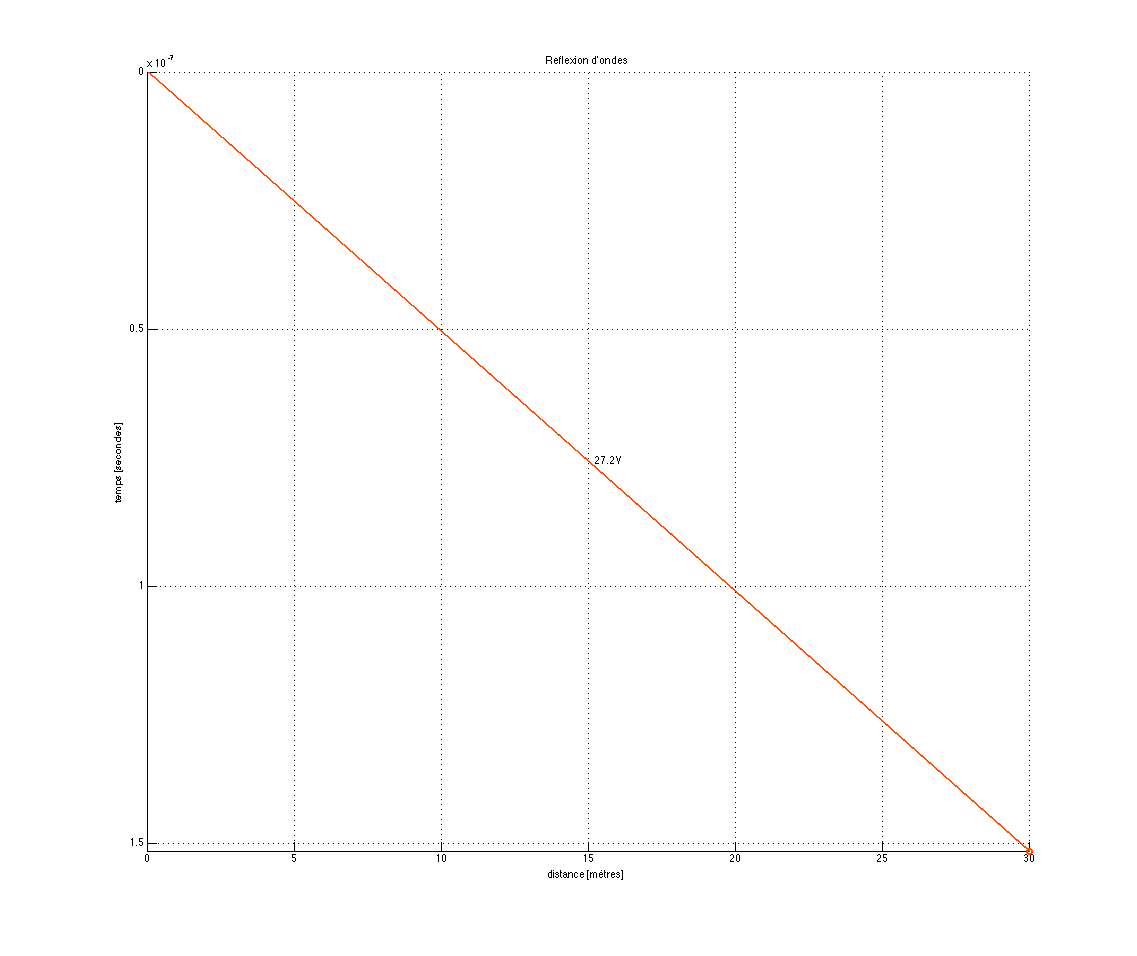
\includegraphics[scale =0.15]{fig/zr50.png} \label{fig:zr50}}
\end{figure}
\clearpage
\newpage
\subsection{Discussion}
La figure \ref{fig:transr0} représente le régime transistoire pour R = 0 $\Omega$ que nous avons mesuré au laboratoire. Lorsque nous comparons avec la figure théorique \ref{fig:r0}, nous remarquons tout de suite la similitude entre les deux courbes. Le signal à la source est atténué complètement après un certain temps. Ceci est causé par la réflexion du signal qui est inversé lorsqu'elle revient. La courbe en Z théorique pour une résistance de 0 Ohm (figure \ref{fig:zr0}) montre bien cet effet. À Z = 0, l'échelon va rencontrer la première droite de 27.2 V au t = 0 ce qui va créer le front montant et par la suite, celui-ci va rencontrer la droite -27.2 V à t = 2T ce qui va créer le front descendant. Le signal vu à la charge peut être analysé de la même façon. Le pic est causé par le signal qui rencontre la droit de 27.2 V à environ Z = 30 et t = T et rencontre la droite de -27.2 V quelques nano-secondes plus tard. Ce pic est bien présent dans les deux figures ce qui valide le modèle utilisé. De plus, selon le calcul de la section 1.2.2, le coefficient de réflexion est de -1 ce qui prouve la forme des courbes obtenues.

\paragraph{} En utilisant la même méthode que précèdemment, il est possible de valider la concordance de la théorie avec la pratique. Selon la courbe en Z théorique pour une résistance de 27 $\Omega$ (figure \ref{fig:zr25}), les courbes vont posséder la même allure que pour R = 0 mais avec des valeurs différentes. Pour la courbe vu de la source, il doit y avoir un échelon de 27.2 V à t = 0 et un échelon de -9 V à t = 2T tandis que pour la courbe vu de la charge, il doit y avoir un échelon d'environ 18 V à t = T. C'est bien ce qui a été obtenu au laboratoire comme il est montré à la figure \ref{fig:transr272}. De plus, il est possible de voir que le régime statique du signal se situe bien à environ 19 V comme le prévoit le coefficient de réflexion de -0.2987. En ce qui concerne le régime transitoire théorique (figure \ref{fig:r27}), celle-ci possèderait les mêmes caractéristiques que la courbe pratique si ce n'était pas du pic à t = T. Ce pic peut-être expliqué par le choix d'afficher la courbe à Z = 29.999 au lieu de 30 car le programme était incapable d'afficher une courbe pour une telle valeur. Comme l'affichage se sert de la courbe en Z, l'échelon passe par la courbe 27.2 à t = T et passe par la courbe de -9 V quelque nano-secondes plus tard comme précédemment.

\paragraph{} Théoriquement, le coefficient de réflexion lorsque la ligne RG-58 est compensé par sa résistance intrinsèque doit être de 0. Le régime transitoire pour un signal avec comme charge une résistance de cet ordre est présenté à la figure \ref{fig:transr501}. En analysant cette figure, il est possible de voir que le coefficient est très proche de 0 car il n'y aucune contribution positive ou négative dû à une réflexion du signal de plus, le délai entre les deux signaux est bien présent ce qui est prévu par la courbe en Z présenté à la figure \ref{fig:zr50}. Tout ce que nous avons sur cette courbe est la droite de 27.2 qui va créer un délai 

\clearpage
\newpage
\section{Projet 3}
La courbe observée à l'oscilloscope est présentée à la figure \ref{CC2}. Le numéro de la charge utilisée est TOEM \#1. On identifie graphiquement une forme de courbe $R-L$ série.  Le $V^{+}$  est de 14V et le 2$V^{+}$ d'environ 27V.

\begin{figure}[htb]
\begin{center}
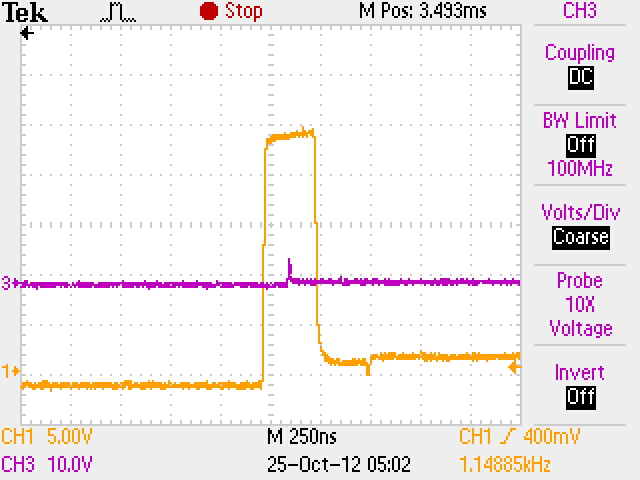
\includegraphics[scale=0.3]{CC2.jpg}
\caption{Courbes obtenus à l'oscilloscope pour le projet 3 en utilisant une charge complexe}
\label{CC2}
\end{center}
\end{figure}

\subsection*{Calcul de R}
En identifiant la valeur finale de la tension (après quelques constantes de temps), on peut déduire la valeur de R conaissant $V^{+}$  et $Z_0$. On utilise l'équation suivante:
\begin{equation}
V_{finale} = V^{+} \left( 1 + \frac{R - Z_0}{R + Z_0}\right)
\end{equation}

On a que $V_{finale} = 3V et Z_0 = 50 \Omega$. On développe l'équation:

\begin{align*}
V_{finale} &= V^{+} \left( 1 + \frac{R - Z_0}{R + Z_0}\right)\\
3 &= 14 \left( 1 + \frac{R - 50}{R + 50}\right)\\
R &= 6 \Omega
\end{align*}

\subsection*{Calcul de $\tau$}

Conaissant maintenant R, on peut trouver $\tau$ au moyen d'un point dans la pente descendante de la courbe, selon l'équation suivante:
\begin{equation}
V_{t\leq \tau} = V^{+} \left( \left(1 + \frac{R - Z_0}{R + Z_0}\right) + \left(1 -\frac{R - Z_0}{R + Z_0}\right) e^{-t/\tau} \right)
\end{equation}

Pour $R=6 \Omega$, $Z_0 = 50 \Omega$ et $V_{t= 250ns} = 16$, on développe l'équation précédente:

\begin{align*}
16 &= 14 \left( \left(1 + \frac{6 - 50}{6 + 50}\right) + \left(1 -\frac{6 - 50}{6 + 50}\right) e^{-250 \times 10^{-9}/\tau} \right)\\
0.5102 &= e^{-250 \times 10^{-9}/\tau}\\
\tau   &= \frac{1}{\frac{ln(0.5102)}{-250 \times 10^{-9}}}\\
\tau   &= 371.497\left[ns\right]
\end{align*}

\subsection*{Calcul de L}

Conaissant maintenant $\tau$, on peut déterminer l'inductance L au moyen de l'équation suivante:
\begin{equation}
\tau = \frac{L}{R + Z_0}
\end{equation}
Pour $R = 6 \Omega$, $Z_0 = 50 \Omega$ et $\tau = 371.497\left[ns\right]$, on développe l'équation précédente:
\begin{align*}
371.497\times 10^{-9} &= \frac{L}{6 + 50}\\
L = 20.8 \left[\mu H\right]
\end{align*}
\newpage
\section{Projet 4}
\subsection{Tracé des régimes transitoires à l'oscilloscope}
\label{s:tracer_transitoire}
Nous avons réalisé le montage pratique tel qu'illustré à la figure 4 de l'énoncé de laboratoire. L'ordre des lignes de transmission a été respecté. Le tracé (à l'oscilloscope) des réponses transitoires obtenues pour des impédances de respectivement 0 $\Omega$, 50 $\Omega$ et 100 $\Omega$ sont présentées aux figures ci-dessous. Il est à noté que le signal vu de la source est sur le canal 1 (orange), que le signal vu à la jonction entre les deux lignes est sur le canal 2 (bleu) et que le signal vu de la charge est sur le canal 3 (vert).

\begin{figure}[htb]
	\centering
\subfigure[Régime transitoire vu de la source, à la jonction entre les lignes et à la charge pour $R = 0 \Omega$]{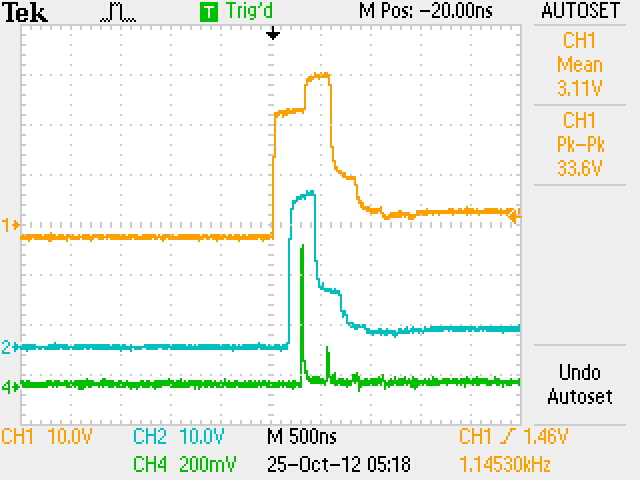
\includegraphics[scale =0.3]{fig/2CRC.JPG} \label{fig:trans2r0}}
		\quad
		\subfigure[Régime transitoire vu de la source, à la jonction entre les lignes et à la charge pour $R = 50 \Omega$]{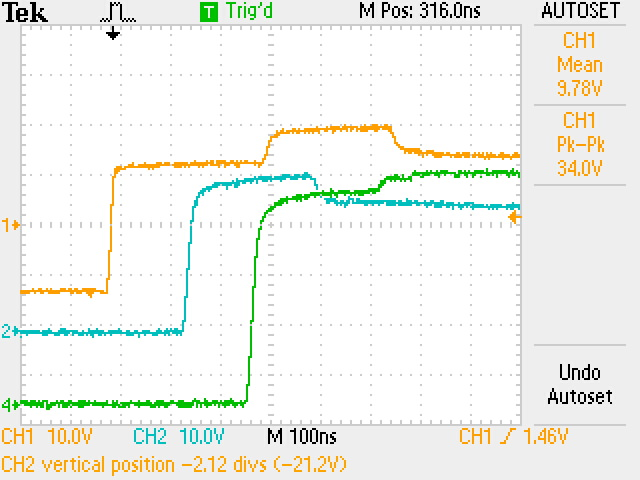
\includegraphics[scale =0.3]{fig/2CR50.JPG} \label{fig:trans2r50}}
		\quad
		\subfigure[Régime transitoire vu de la source, à la jonction entre les lignes et à la charge pour $R = 100 \Omega$]{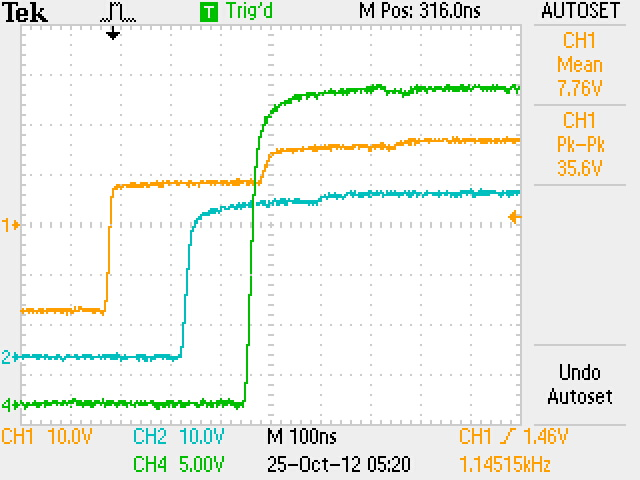
\includegraphics[scale =0.3]{fig/2CR100.JPG} \label{fig:trans2r100}}
\end{figure}
\newpage
\subsection{Calcul du coefficient de réflexion à la source}
Pour calculer le coefficient de réflexion à la source, on utilise l'équation \ref{eq:reflex} en sachant qu'elle sera la même peu importe la charge:
\begin{align*}
\Gamma_g (s) &= \frac{50 - 50}{50 + 50}\\
&= 0
\end{align*}
\subsection{Calcul du coefficient de réflexion du côté de la ligne \# 1}
On définit l'équation suivante et on la développe selon les valeurs connues
\begin{align}
\Gamma_{11} &= \frac{Z_{02} - Z_{01}}{Z_{02} + Z_{01}}\\
			&= \frac{93-50}{93 + 50}\notag\\
			&= 0.3007\notag
\end{align}
\subsection{Calcul du coefficient de réflexion du côté de la ligne \# 2}
On définit l'équation suivante et on la développe selon les valeurs connues
\begin{align}
\Gamma_{22} &= \frac{Z_{01} - Z_{02}}{Z_{01} + Z_{02}}\\
			&= \frac{50-93}{93 + 50}\notag\\
			&= -0.3007\notag
\end{align}
\subsection{Calcul des coefficients de réflexion du côté des charges}
\textbf{Pour R = $0\Omega$}
\begin{align*}
\Gamma_c (s) &= \frac{Z_c(s) - Z_0(s)}{Z_c(s) + Z_0(s)}\\
			 &= \frac{0 - 93 }{0 + 93}\\
			 &= -1
\end{align*}
\textbf{Pour R = $50\Omega$}
\begin{align*}
\Gamma_c (s) &= \frac{Z_c(s) - Z_0(s)}{Z_c(s) + Z_0(s)}\\
			 &= \frac{50 - 93 }{93 + 50}\\
			 &= -0.3007
\end{align*}
\textbf{Pour R = $100\Omega$}
\begin{align*}
\Gamma_c (s) &= \frac{Z_c(s) - Z_0(s)}{Z_c(s) + Z_0(s)}\\
			 &= \frac{100 - 93 }{100 + 93}\\
			 &= 0.0363
\end{align*}
\subsection{Calcul du coefficient de transmission de la ligne \# 1 vers la ligne \# 2}
On définit l'équation suivante et on la développe selon les valeurs connues
\begin{align}
\tau_{12} &= (1-\Gamma_{11})\\
			&= 1 - 0.3007\notag\\
			&= 0.6993\notag
\end{align}
\subsection{Calcul du coefficient de transmission de la ligne \# 2 vers la ligne \# 1}
On définit l'équation suivante et on la développe selon les valeurs connues
\begin{align}
\tau_{21} &= (1-\Gamma_{22})\\
			&= 1 + 0.3007\notag\\
			&= 1.3007\notag
\end{align}
\subsection{Régimes transitoires théoriques }

\begin{figure}[htb]
	\centering
\mbox{\subfigure[Régime transitoire théorique vu de la source, à la jonction entre les lignes et à la charge pour $R = 0 \Omega$]{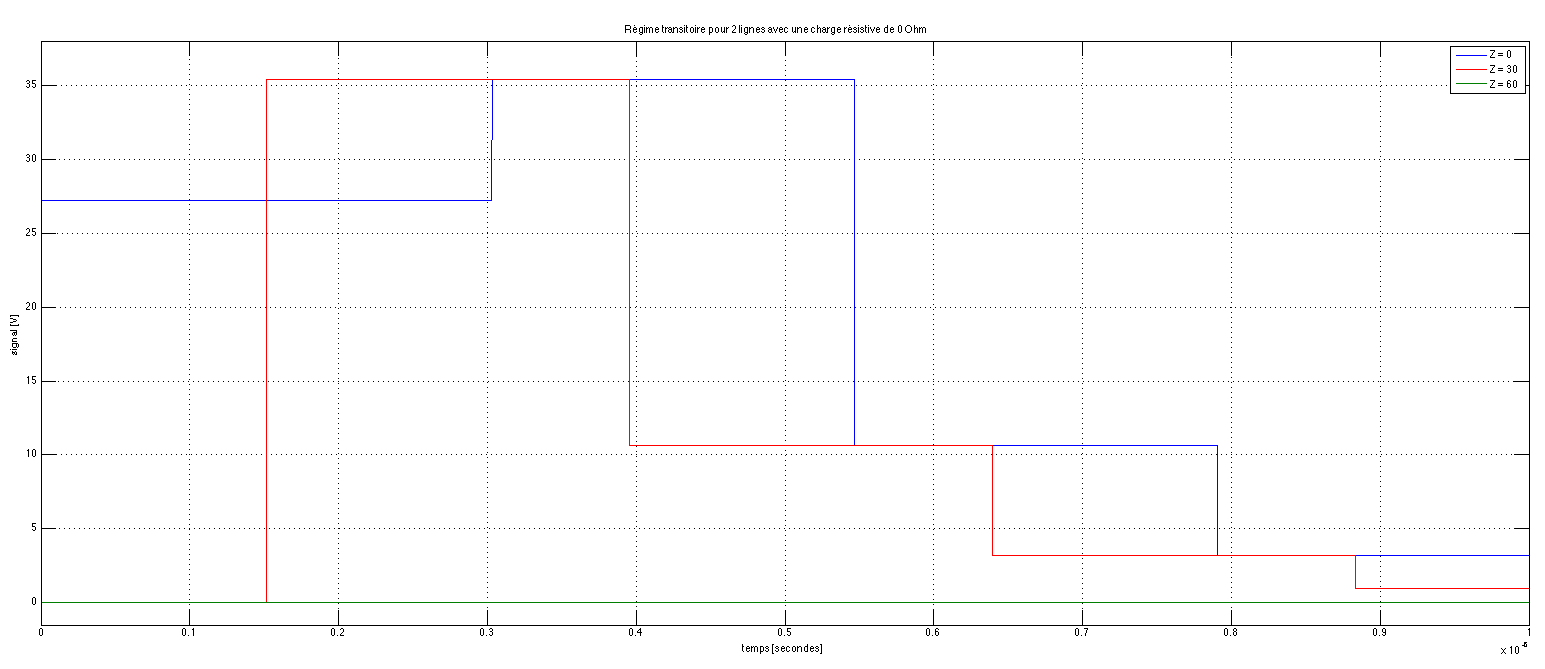
\includegraphics[scale =0.3]{fig/2r0.png} \label{fig:2r0}}}
\end{figure}



\begin{figure}[htb]
	\centering
	\mbox{\subfigure[Régime transitoire théorique vu de la source, à la jonction entre les lignes et à la charge pour $R = 50 \Omega$]	{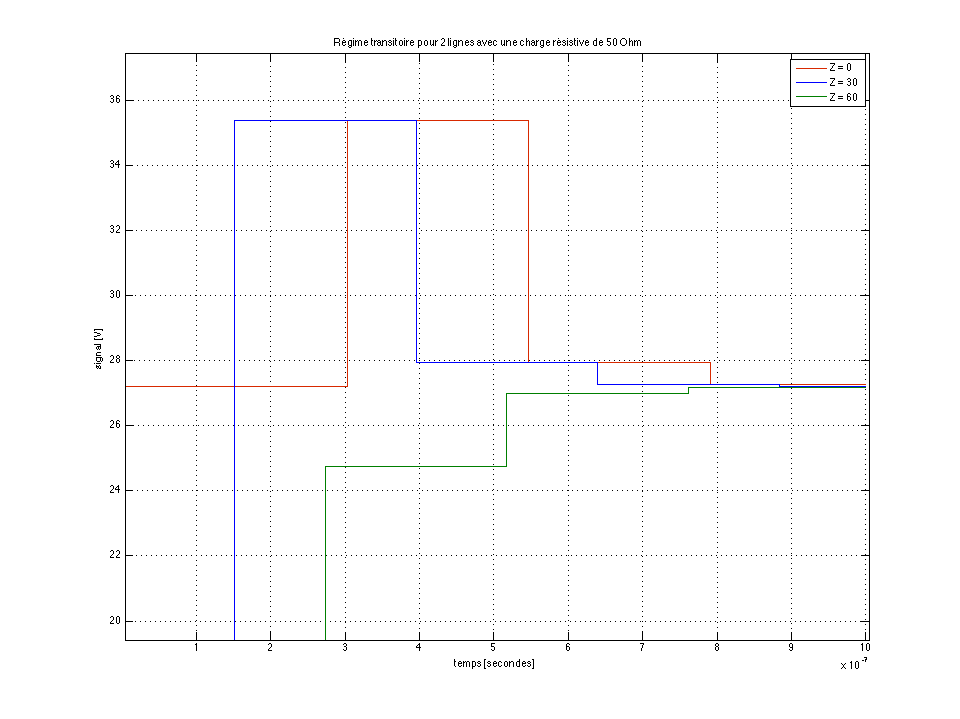
\includegraphics[scale =0.25]{fig/2r50.png} \label{fig:2r50}}
		\subfigure[Régime transitoire théorique vu de la source, à la jonction entre les lignes et à la charge pour $R = 100 \Omega$]{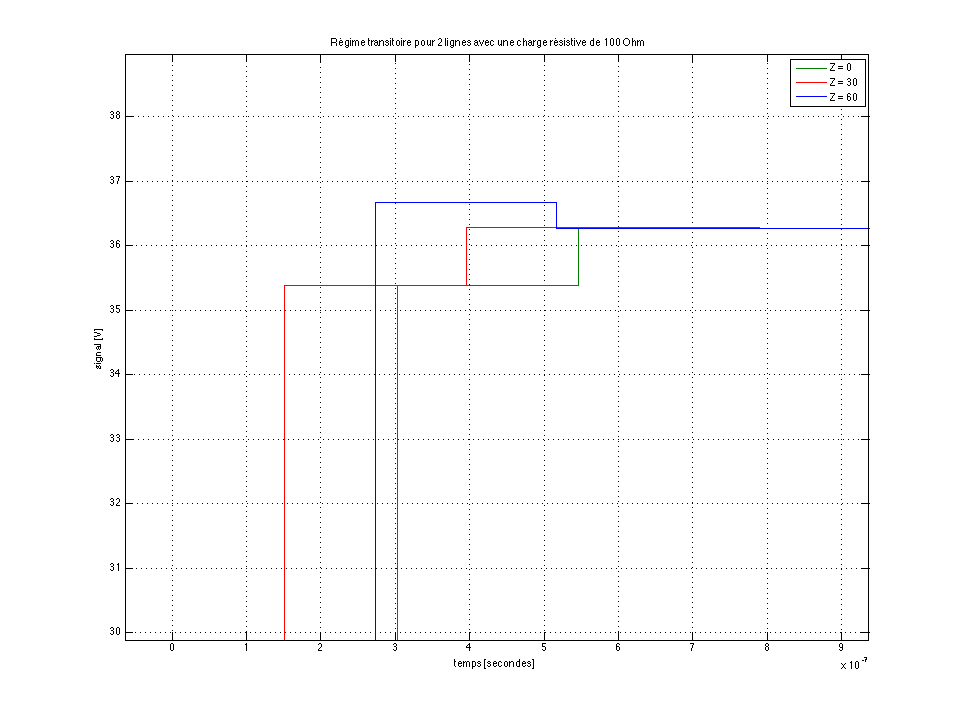
\includegraphics[scale =0.25]{fig/2r100.png} \label{fig:2r100}}}
\end{figure}


\subsection{Diagrammes en z}

\begin{figure}[htb]
	\centering
	\mbox{\subfigure[Diagramme en z pour $R = 0 \Omega$]{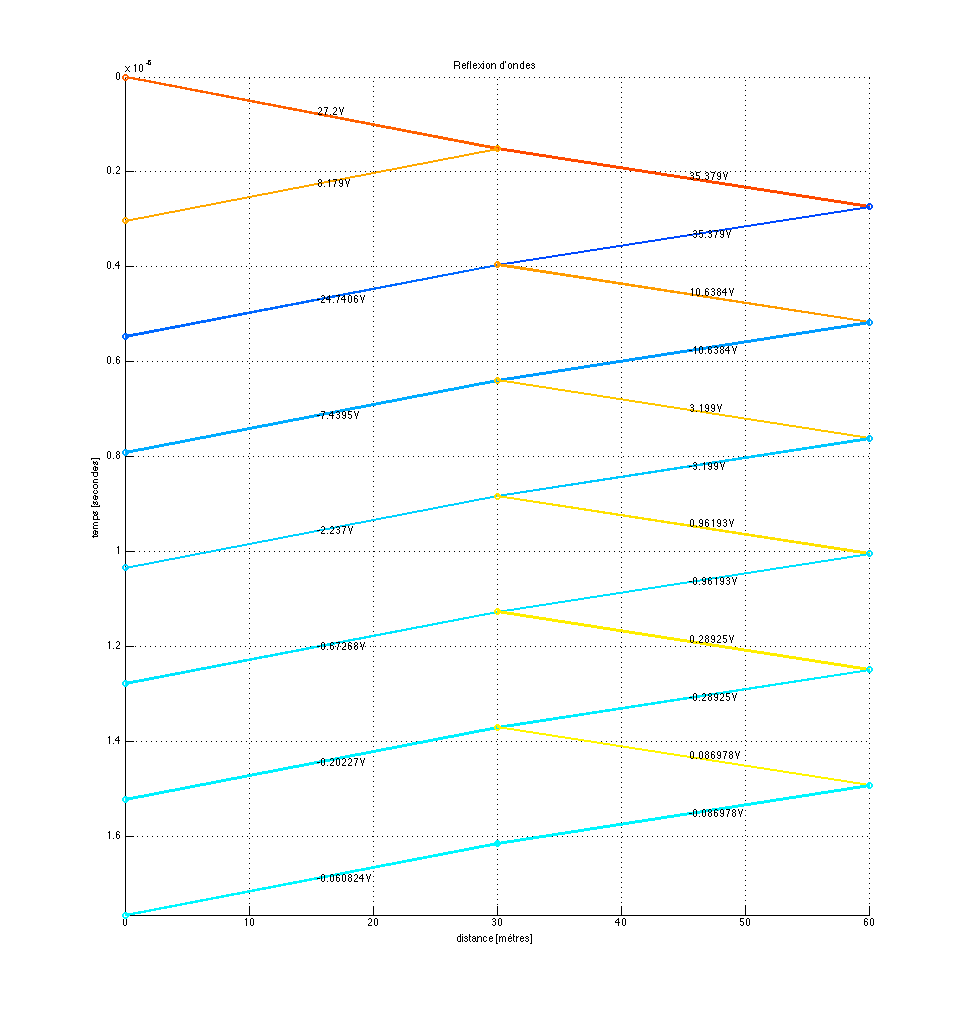
\includegraphics[scale =0.25]{fig/2zr0.png} \label{fig:2zr0}}
		\subfigure[Diagramme en z pour $R = 50 \Omega$]{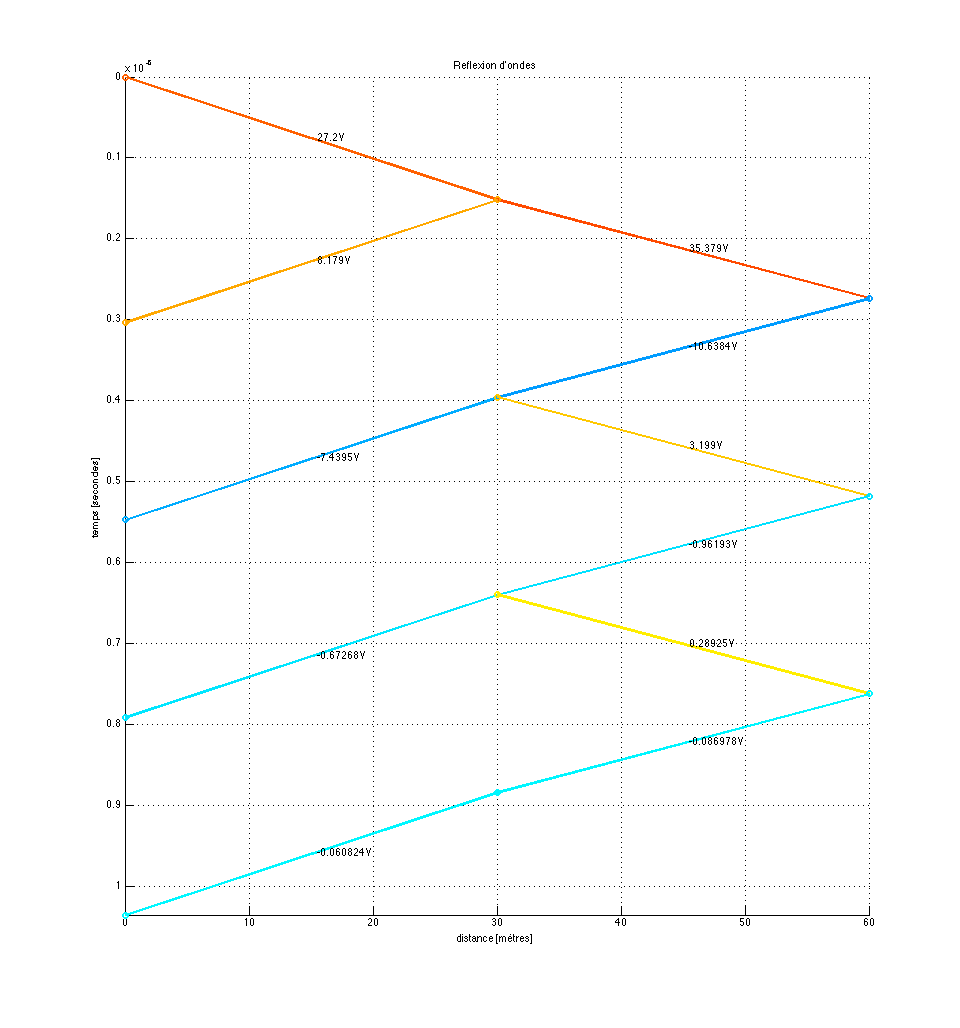
\includegraphics[scale =0.25]{fig/2zr50.png} \label{fig:2zr50}}}
\end{figure}

\begin{figure}[htb]
	\centering
	\mbox{\subfigure[Diagramme en z pour $R = 100 \Omega$]{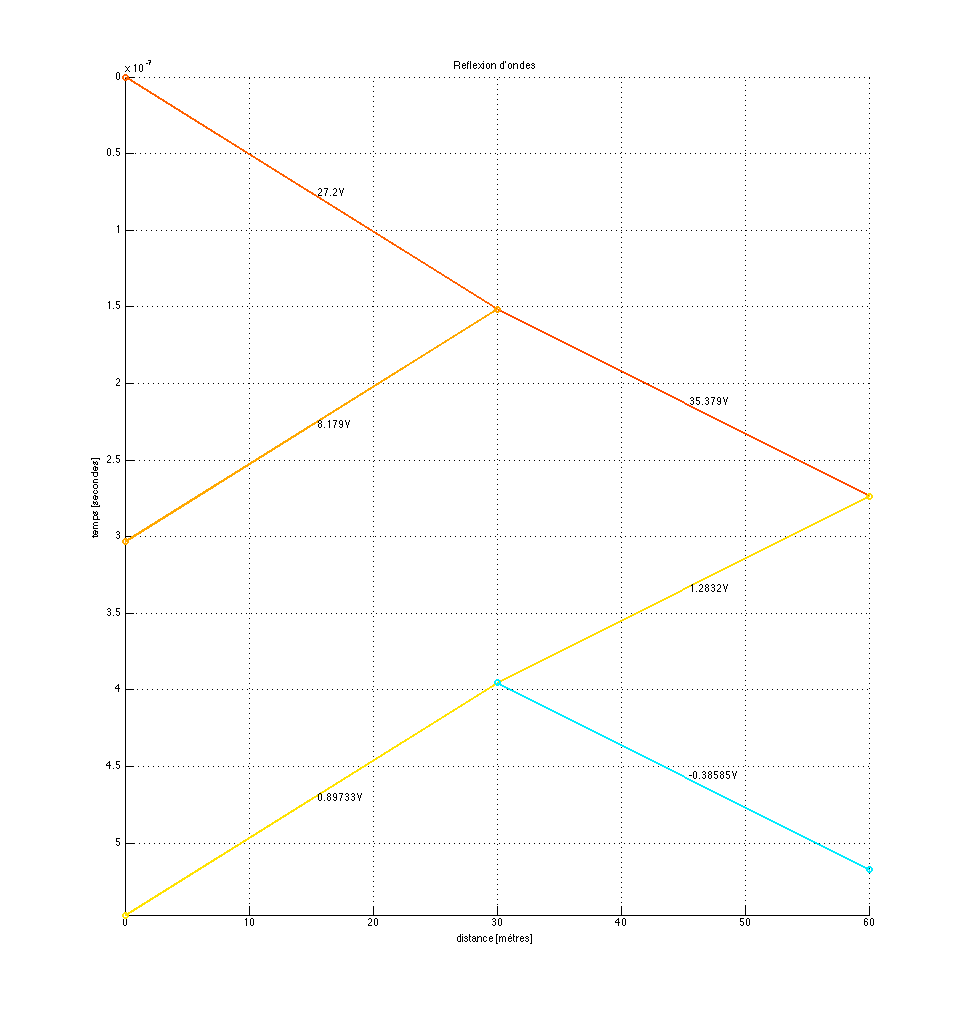
\includegraphics[scale =0.25]{fig/2zr100.png} \label{fig:2zr100}}}
\end{figure}
\clearpage
\newpage

\subsection{Discussion}

\subsubsection{Régime transitoire}
Les figures \ref{fig:trans2r0}, \ref{fig:trans2r50} et \ref{fig:trans2r100} présentent les régimes transitoires pour diverses charges. Le code de couleur utilisé est toujours le même, tel que présenté à la section \ref{s:tracer_transitoire}. Les figures \ref{fig:2r0}, \ref{fig:2r50} et \ref{fig:2r100} présentent le pendant théorique des courbes mesurées expérimentalement. Pour ce qui est des courbes présentant le comportement du système avec une résistance $R=0\Omega$, on note premièrement que la courbe théorique relatant le comportement de la tension vue à la source (la courbe bleue) suit le même comportement que celle mesurée expérimentalement. En dehors des limitations physiques de la source de tension, l'incurvation de la courbe expérimentale s'explique par la limite en bande passante de l'oscilloscope ainsi que par la présence d'impédances complexes dans le circuit. 

\paragraph{}Pour ce qui est de la tension vue à la première jonction, on remarque que le comportement est similaire à la théorie. Cependant, le système étudié présente les mêmes limitations. 

\paragraph{}On ne réussit malheureusement pas à afficher une courbe montrant la tension vue aux bornes de la charge, cependant, comme la montée théorique est très rapide et fait intervenir le comportement aux limites du logiciel, il est comprenable qu'il soit difficile de l'afficher. 

\paragraph{}En ce qui concerne la résistance de $50\Omega$, le comportement est pratiquement similaire en tous points. Les transitions mesurées expérimentalement sont moins brusques, mais il est possible de déceler une forte corrélation entre les mesures expérimentale et la théorie. 

\paragraph{}Les courbes présentant le régime transitoire pour une résistance de $100\Omega$ sont en tous points identiques. On voit que le modèle théorique prédit bien le comportement observé au laboratoire. 
\subsubsection{Diagrammes en z}

Les figures \ref{fig:2zr0}, \ref{fig:2zr50} et \ref{fig:2zr100} présentent le diagramme en z pour différentes résistances placées en fin de ligne. On note que le minimum de réflexion est atteint pour une résistance de $100\Omega$. La résistance de $0\Omega$ présente le nombre le plus élevé de réflexions, ce qui était prédit par les calculs et la théorie vue au cours. La résistance de $50\Omega$ fournit un indice de réflexion mitoyen entre les deux valeurs extrêmes de résistance. Le nombre de réflexion est plus faible que celui avec une résistance de $0\Omega$, mais plus élevé que celui avec une résistance de $100\Omega$. 

\section{Conclusion}

Les projets 1 à 4 témoignent de la véracité du modèle étudié. Les similitudes entre la théorie et l'expérimentation montrent que le modèle étudié est suffisant pour prédire le comportement expérimental des réflexions dans une ligne de transmission avec une ou plusieurs jonctions. Nous avons pu faire l'analyse transitoire des signaux pour différentes valeurs de résistance de charge et ainsi, vérifier les équations entourant les coefficients de réflexions ainsi que le modèle expérimental.  Nous avons montré qu'il est possible d'identifier les différents paramètres d'une charge réactive en bout de ligne au moyen du projet 3. Aussi, lors du dernier projet, il fut possible de vérifier l'impact de l'ajout d'une jonction sur la forme des signaux à la source et aux différentes jonctions. De ce fait, il fut possible d'en tracer les diagrammes en z ainsi que les diagrammes théoriques associés, de manière à mieux saisir le comportement observé. L'ensemble du laboratoire nous a permis de nous familiarisé avec la théorie et d'en comprendre les implications pratiques. 

%%!TEX root = ../rapport.tex
%!TEX encoding = UTF-8 Unicode
\chapter{Expérimentation, Analyse, Résultat}


%%!TEX encoding = UTF-8 Unicode
%!TEX root = ../rapport.tex
% Chapitres "Conclusion"

% modifié par Francis Valois, Université Laval
% 31/01/2011 - version 1.0 - Création du document

\chapter{Conclusion}
\label{s:conclusion}

Au cours de ce septième laboratoire, nous nous sommes familiarisé avec l'implantation pratique d'un oscillateur triangulaire pouvant être employé afin de moduler un signal quelconque. Par ailleurs, nous nous sommes aussi familiarisé avec l'implantation d'un comparateur à hystérésis capable d'effectuer ladite modulation en procurant une protection additionnelle contre le buit. Aussi, nous avons su implanté de manière pratique un filtre Butterworth d'ordre 2 ayant pour fonction d'effectuer la démodulation du signal. De par la précision la similitude entre l'onde de sortie et l'onde d'entrée, nous avons pu constater l'efficacité de notre montage et les qualités de la réponse en fréquence du filtre Butterworth. Il est intéressant de noter le déphasage des signaux de sortie, déphasage tout de même significatif, qui provient de la fonction de filtrage qui induit un déphasage non nul dans sa fonction de transfert.

\appendix
%%!TEX root = ../rapport.tex
%!TEX encoding = UTF-8 Unicode
% Chapitres "Annexes"

% modifié par Francis Valois, Université Laval
% 31/01/2011 - version 1.0 - Création du document
\chapter{Projet 1}
\label{s:annexes}

\begin{figure}[htb]
	\centering
\subfigure[Courbes de réflexion obtenue pour $R = 0\Omega$]{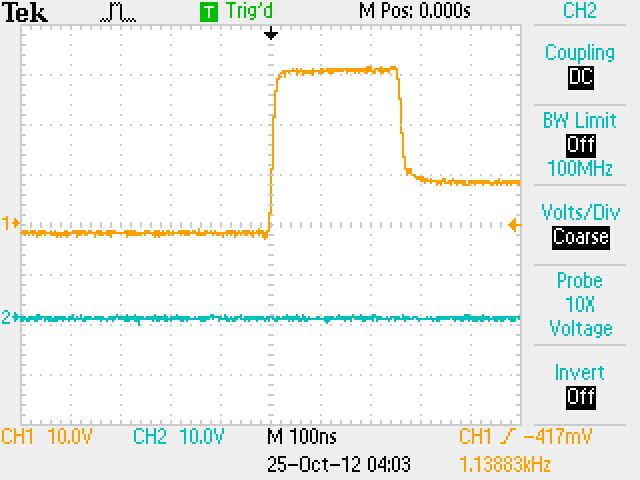
\includegraphics[scale =0.3]{fig/RR0.JPG} \label{fig:reflexr0}}
		\quad
		\subfigure[Courbes de réflexion obtenue pour $R = 27\Omega$]{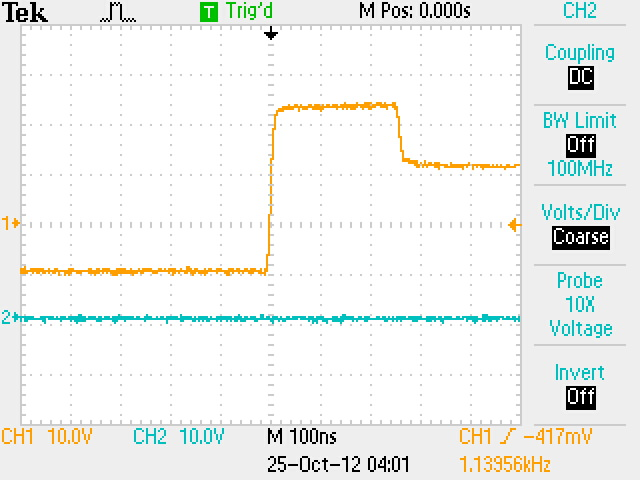
\includegraphics[scale =0.3]{fig/RR27.JPG} \label{fig:reflexr27}}
		\quad
		\subfigure[Courbes de réflexion obtenue pour $R = 50\Omega$]{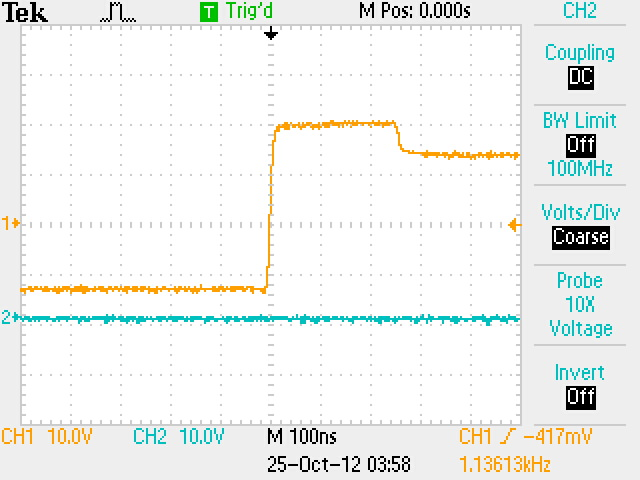
\includegraphics[scale =0.3]{fig/RR50.JPG} \label{fig:reflexr50}}
		\quad
		\subfigure[Courbes de réflexion obtenue pour $R = \infty$]{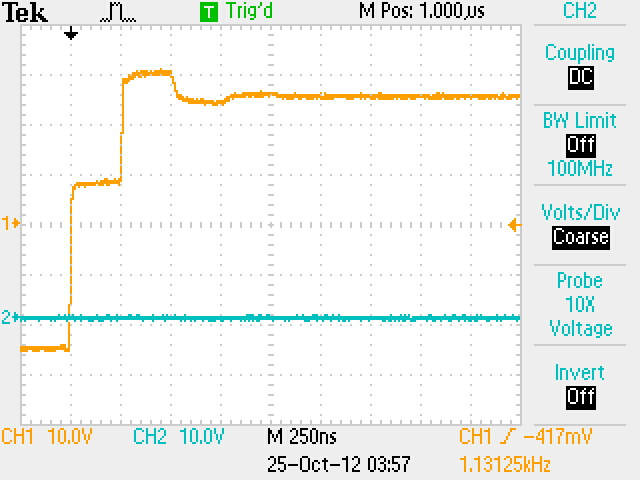
\includegraphics[scale =0.3]{fig/RRCO.JPG} \label{fig:reflexrco}}
\end{figure}




\end{document}
% Fin du document

